
%(BEGIN_QUESTION)
% Copyright 2008, Tony R. Kuphaldt, released under the Creative Commons Attribution License (v 1.0)
% This means you may do almost anything with this work of mine, so long as you give me proper credit

Determine what will happen to the following voltage drops (between specified test points in the circuit) if the resistance of resistor $R_3$ happens to decrease:

$$\includegraphics[width=15.5cm]{i02914x01.eps}$$

\begin{itemize}
\item{} $V_{AC}$ = ({\it increase}, {\it decrease}, or {\it stay the same})
\vskip 10pt
\item{} $V_{BE}$ = ({\it increase}, {\it decrease}, or {\it stay the same})
\vskip 10pt
\item{} $V_{AD}$ = ({\it increase}, {\it decrease}, or {\it stay the same})
\vskip 10pt
\item{} $V_{CD}$ = ({\it increase}, {\it decrease}, or {\it stay the same})
\end{itemize}

\vfil 

\underbar{file i02914}
\eject
%(END_QUESTION)





%(BEGIN_ANSWER)

This is a graded question -- no answers or hints given!

%(END_ANSWER)





%(BEGIN_NOTES)

A key observation to make is that the current through $R_4$ and $R_5$ will increase as the resistance of $R_3$ decreases.

\begin{itemize}
\item{} $V_{AC}$ = {\bf decrease}
\vskip 10pt
\item{} $V_{BE}$ = {\bf increase}
\vskip 10pt
\item{} $V_{AD}$ = {\bf stay the same}
\vskip 10pt
\item{} $V_{CD}$ = {\bf increase}
\end{itemize}

A good problem-solving technique to use here is {\it limiting cases}.  Instead of merely considering the effects of a resistance changing slightly, we imagine that resistance suffering an extreme change (e.g. an increasing resistance gets viewed as an ``open,'' while a decreasing resistance gets viewed as a dead short -- both ``limiting cases'' of the given trend).  The circuit will become simpler is we analyze it under such an extreme condition, and the directions of the changes in a linear DC circuit such as this will be the same as for a milder change.

Another good problem-solving technique is to assume simple values for each resistor (say, 1 k ohm) and a simple voltage source value, then actually perform quantitative calculations to see what happens in the event of the limiting-case component change.  The last answer might best be arrived at in this manner.

\vskip 10pt

Yet another applicable problem-solving technique is to {\it re-draw the circuit} so that it is easier to analyze.  Something like this may be helpful:

$$\includegraphics[width=15.5cm]{i02914x02.eps}$$

%INDEX% Electronics review: qualitative analysis of DC series-parallel resistor circuit

%(END_NOTES)


